\section{Results}
\label{sec:results}

The data is displayed in the plane of \MET\ vs. \Ht\ in Fig.~\ref{fig:met_ht}.
We find 4 (3) events in the high \MET\ (high \Ht) signal regions, consistent
with the MC expectations. 

\begin{figure}[tbh]
\begin{center}
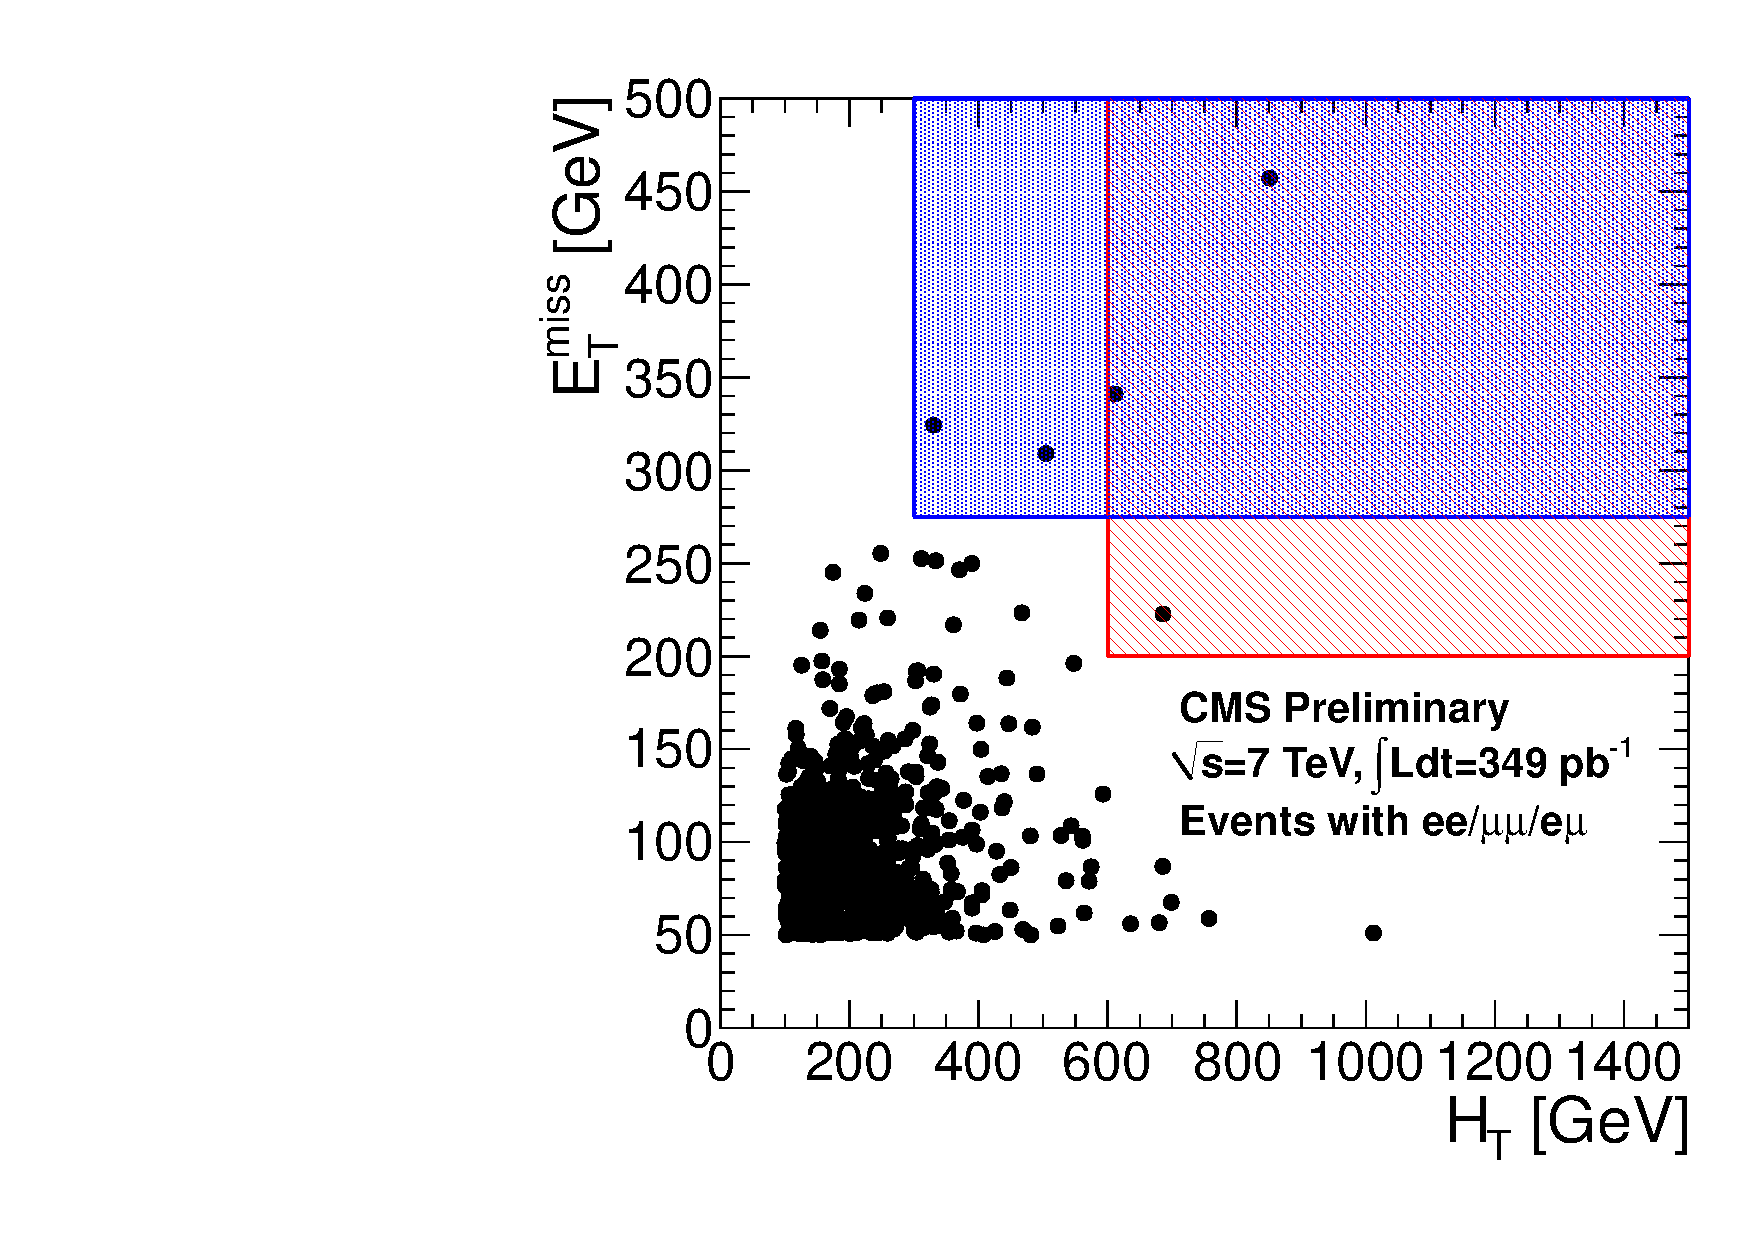
\includegraphics[width=0.65\linewidth]{plots_final/met_ht_349pb.pdf}
\caption{\label{fig:met_ht}\protect Distributions of \MET\ vs.\ \HT\   
for data. The high \MET\ (high \Ht) signal region is indicated with the
blue dotted (red striped) region.}
\end{center}
\end{figure}

Next, we apply the ABCD' method to predict the yields in the high \met\ and high \Ht\
signal regions. The $y$ vs. \Ht\ distributions for data are displayed in 
Fig.~\ref{fig:abcdprimedata}. The signal regions are indicated, as well as the control 
regions used to measure the $f(y)$ and $g(H_T)$ distributions. For the high \met\
signal region, we find a predicted yield of 1.2 $\pm$ 0.4 (stat) $\pm$ 0.5 (syst), 
in reasonable agreement with the MC prediction. For the high \Ht\ signal region, we 
do not find any events in the control region used to extract $g(H_T)$ with \Ht\ $>$ 600 GeV,
and the ABCD' background estimate is therefore 0. To assess the statistical uncertainty
in this prediction, we add a single event ``by hand'' to the $g(H_T)$ distributiion
at $H_T = 600$ GeV, leading to a predicted yield of 0.0 $\pm$ 0.6 (stat) $\pm$ 0.3 (syst).


\begin{figure}[hbt]
\begin{center}
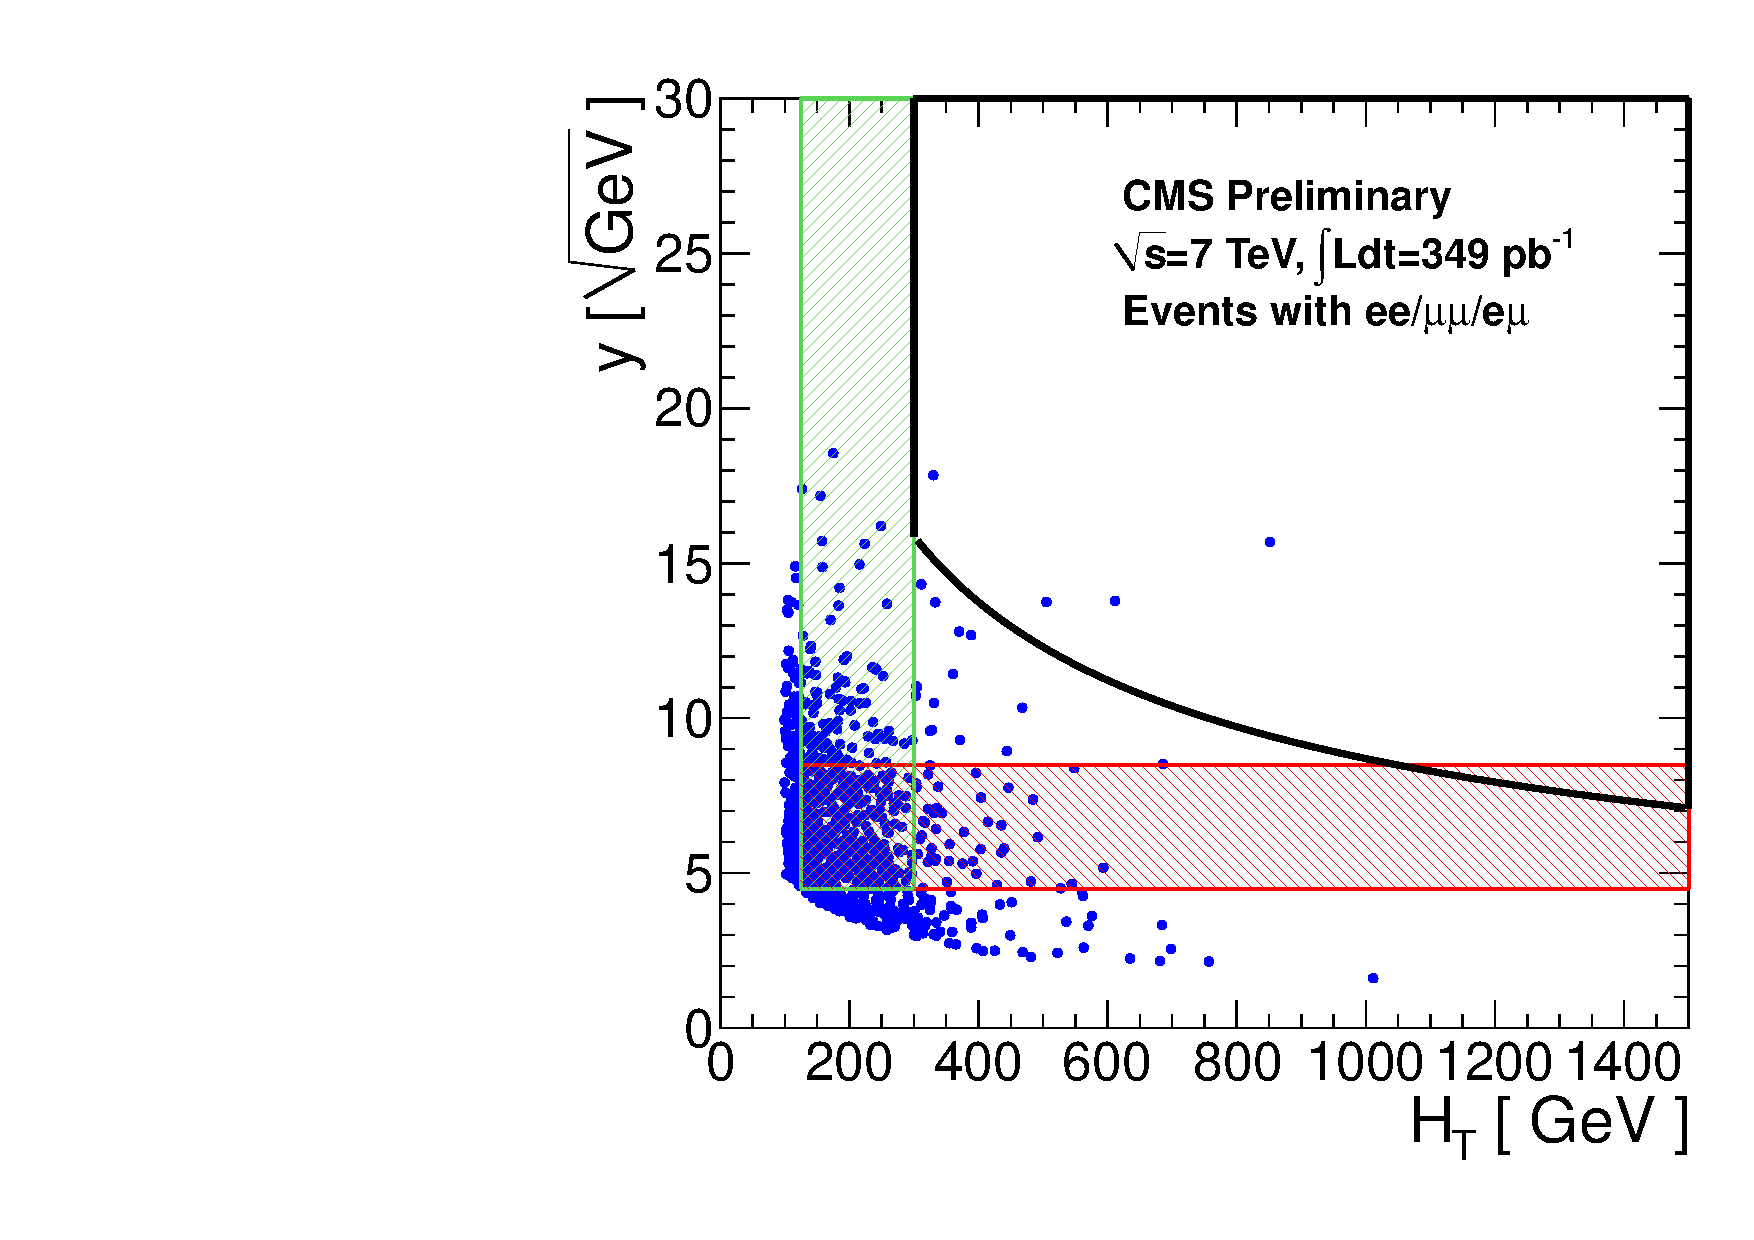
\includegraphics[width=0.48\linewidth]{plots_final/abcdprime_349pb_highmet.pdf}
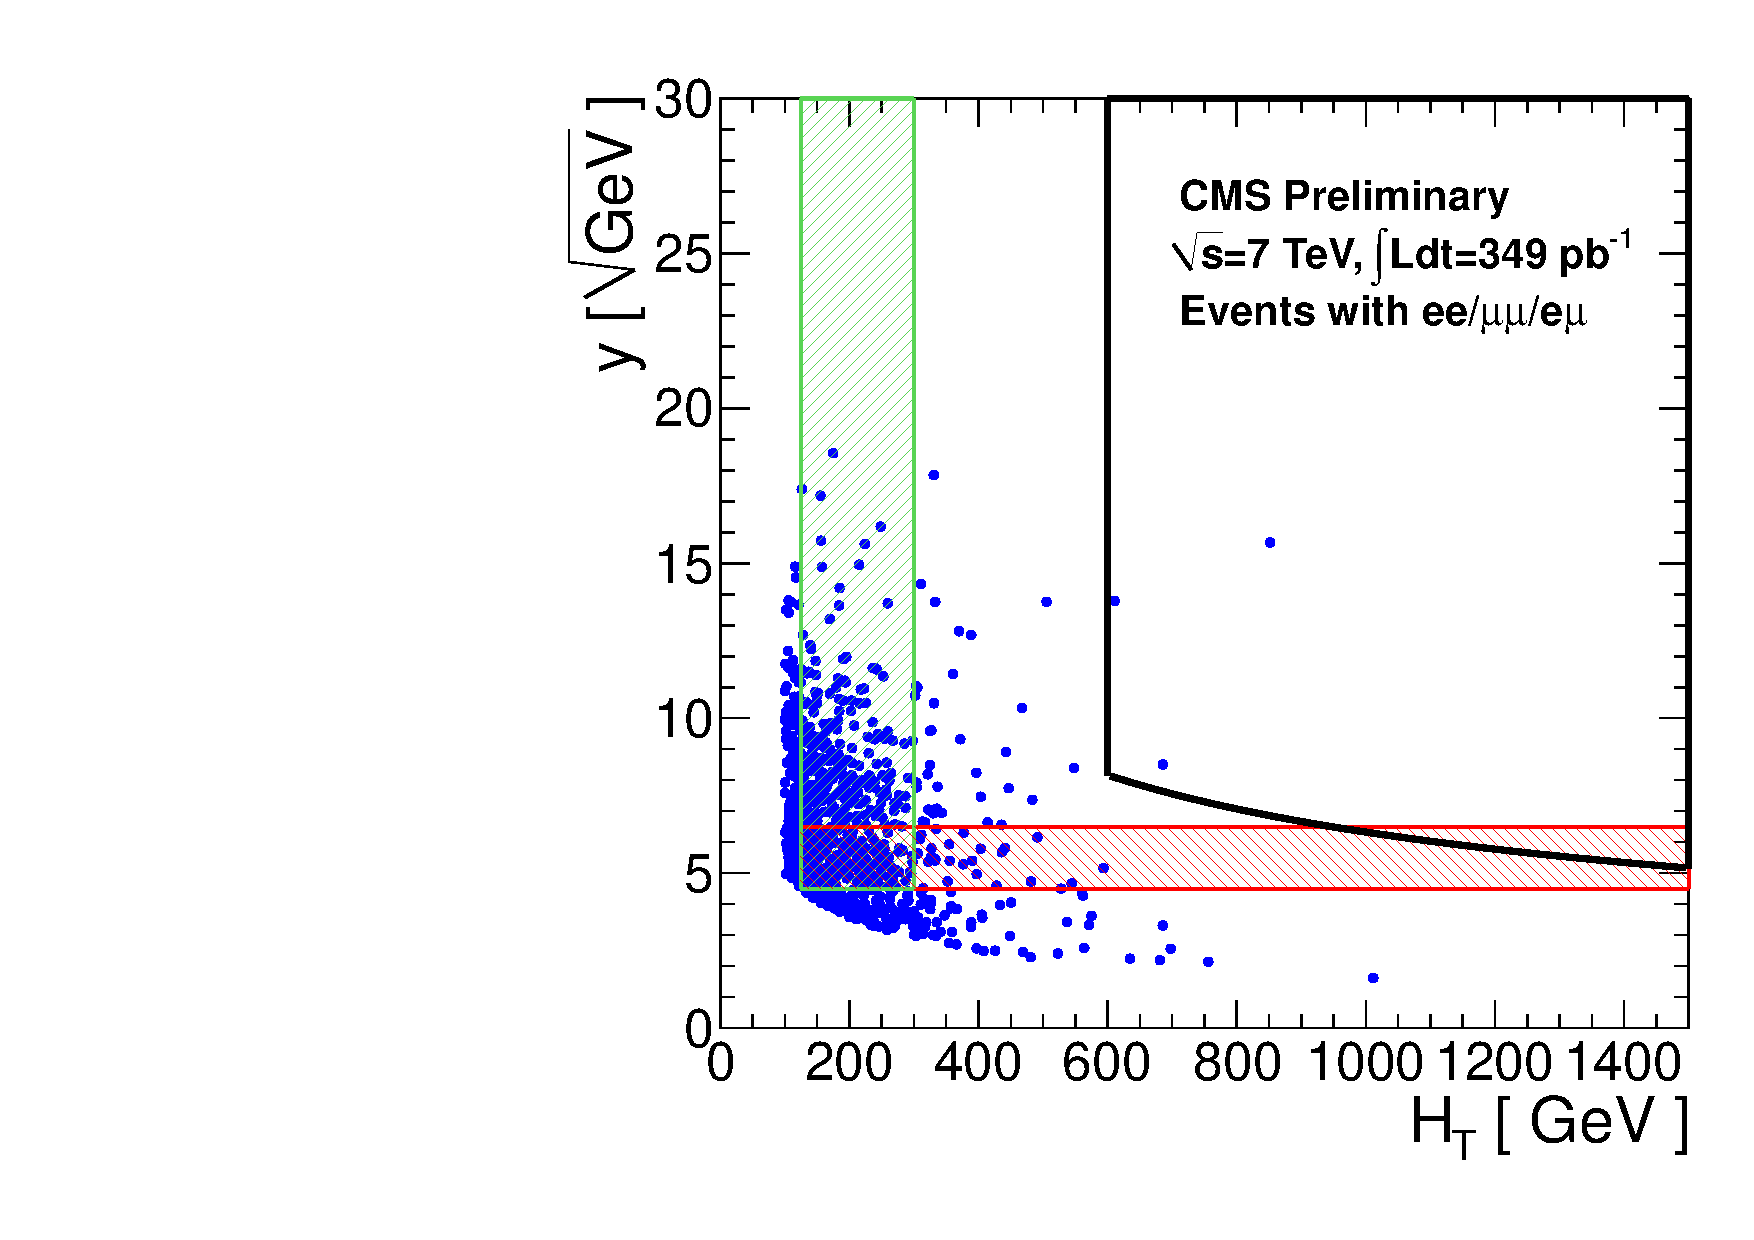
\includegraphics[width=0.48\linewidth]{plots_final/abcdprime_349pb_highht.pdf}
\caption{\label{fig:abcdprimedata}\protect 
Distributions of $y$ vs. \Ht\ in data. The signal regions \met\ $>$ 275 GeV, \Ht\ $>$ 300 GeV (left)
and \met\ $>$ 200 GeV, \Ht\ $>$ 600 GeV (right) are indicated with thick black lines. 
The $f(y)$ and $g(H_T)$ 
functions are measured using events in the green and red shaded areas, respectively.
}
\end{center}
\end{figure}

Next, we use the \ptll\ template method to predict the background in the 2 signal regions.
For each signal region D, we count the number of events falling in the region D', which is 
defined using the same requirements as D but replacing the \MET\ requirement with a \ptll\
requirement. We subtract off the expected DY contribution using the data-driven $R_{out/in}$
technique. We scale this yield by 2 corrections factors: $K$, the \met\ acceptance 
correction factor, and $K_C$, the correction factor determined in Sec.~\ref{sec:datadriven}.
Our final prediction $N_P$ is given by:

\begin{center}
$ N_P = (N(D')-N(DY)) \times K \times K_C$.
\end{center}


\begin{figure}[hbt]
\begin{center}
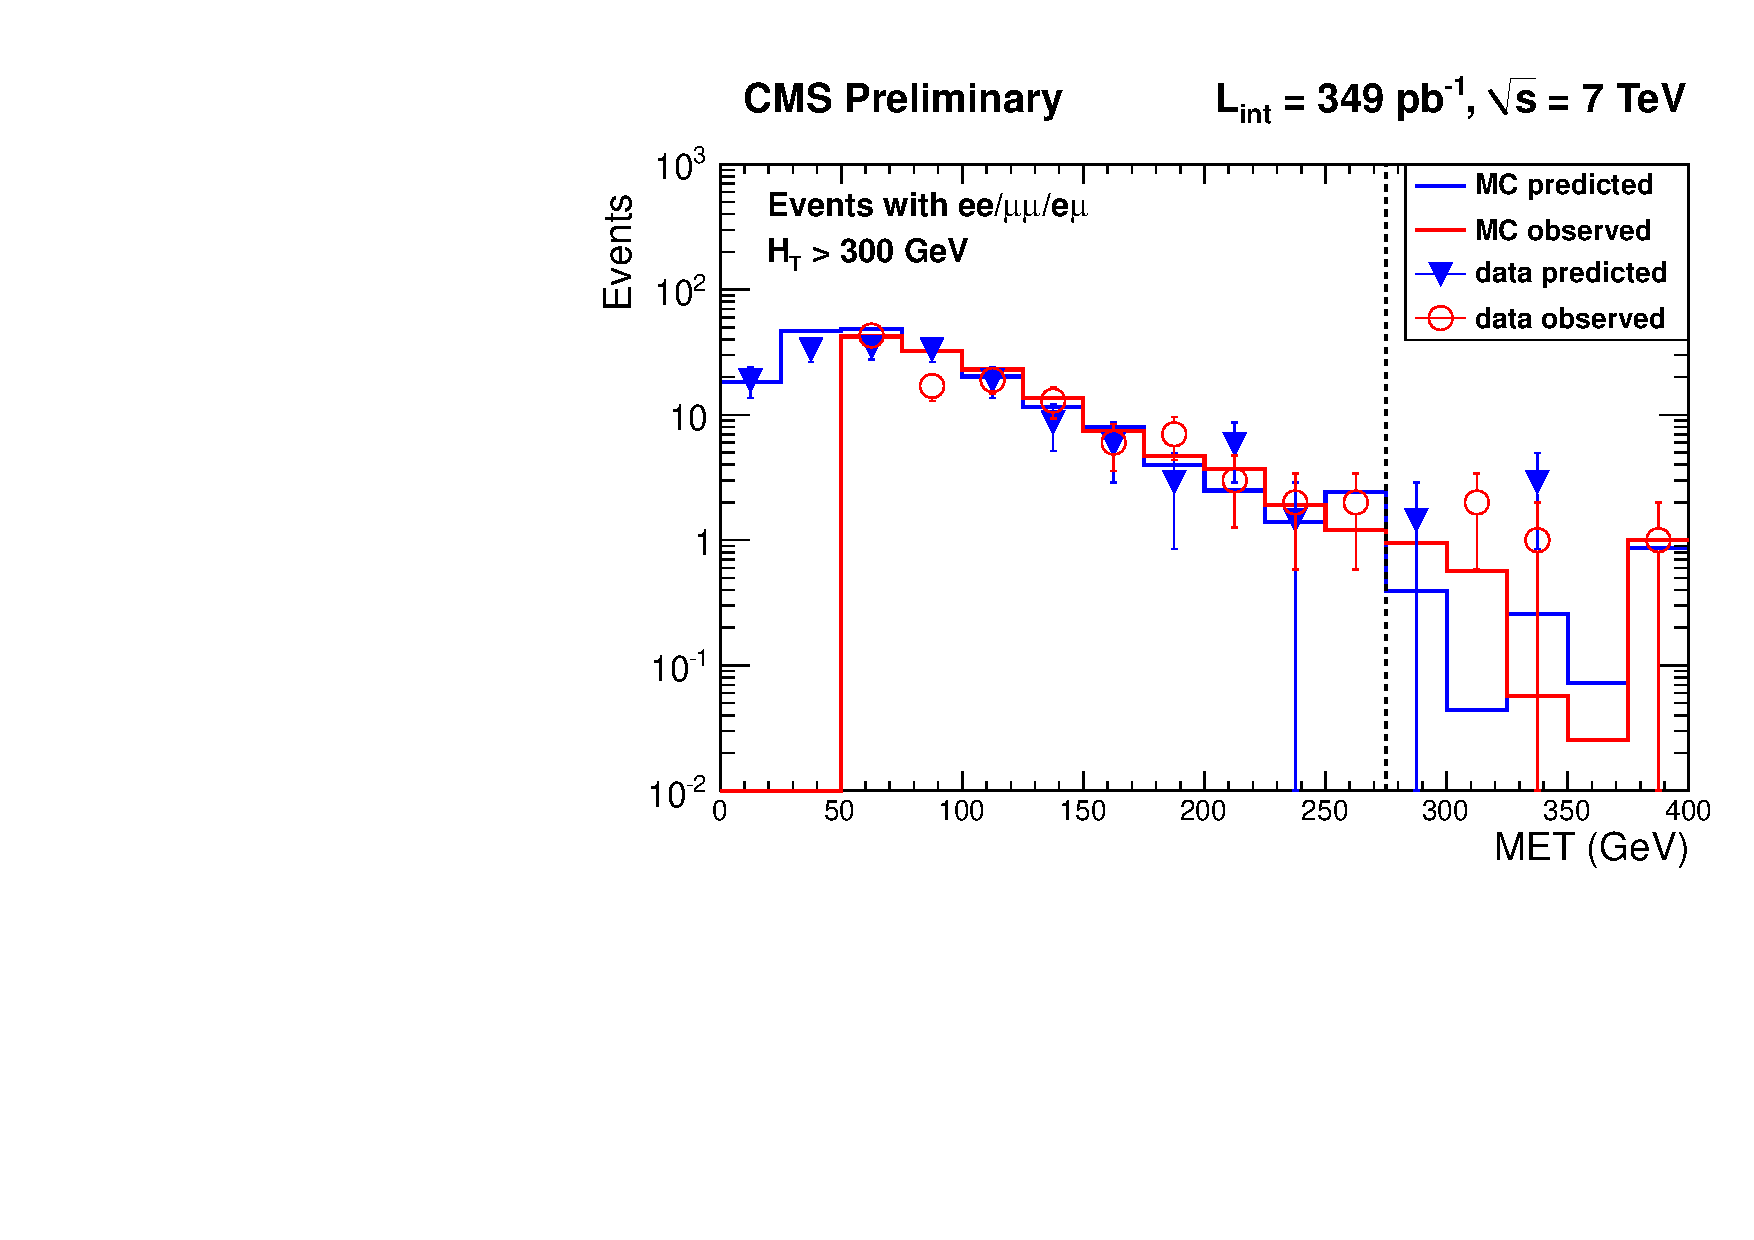
\includegraphics[width=0.48\linewidth]{plots_final/victory_met275_ht300_349pb.pdf}
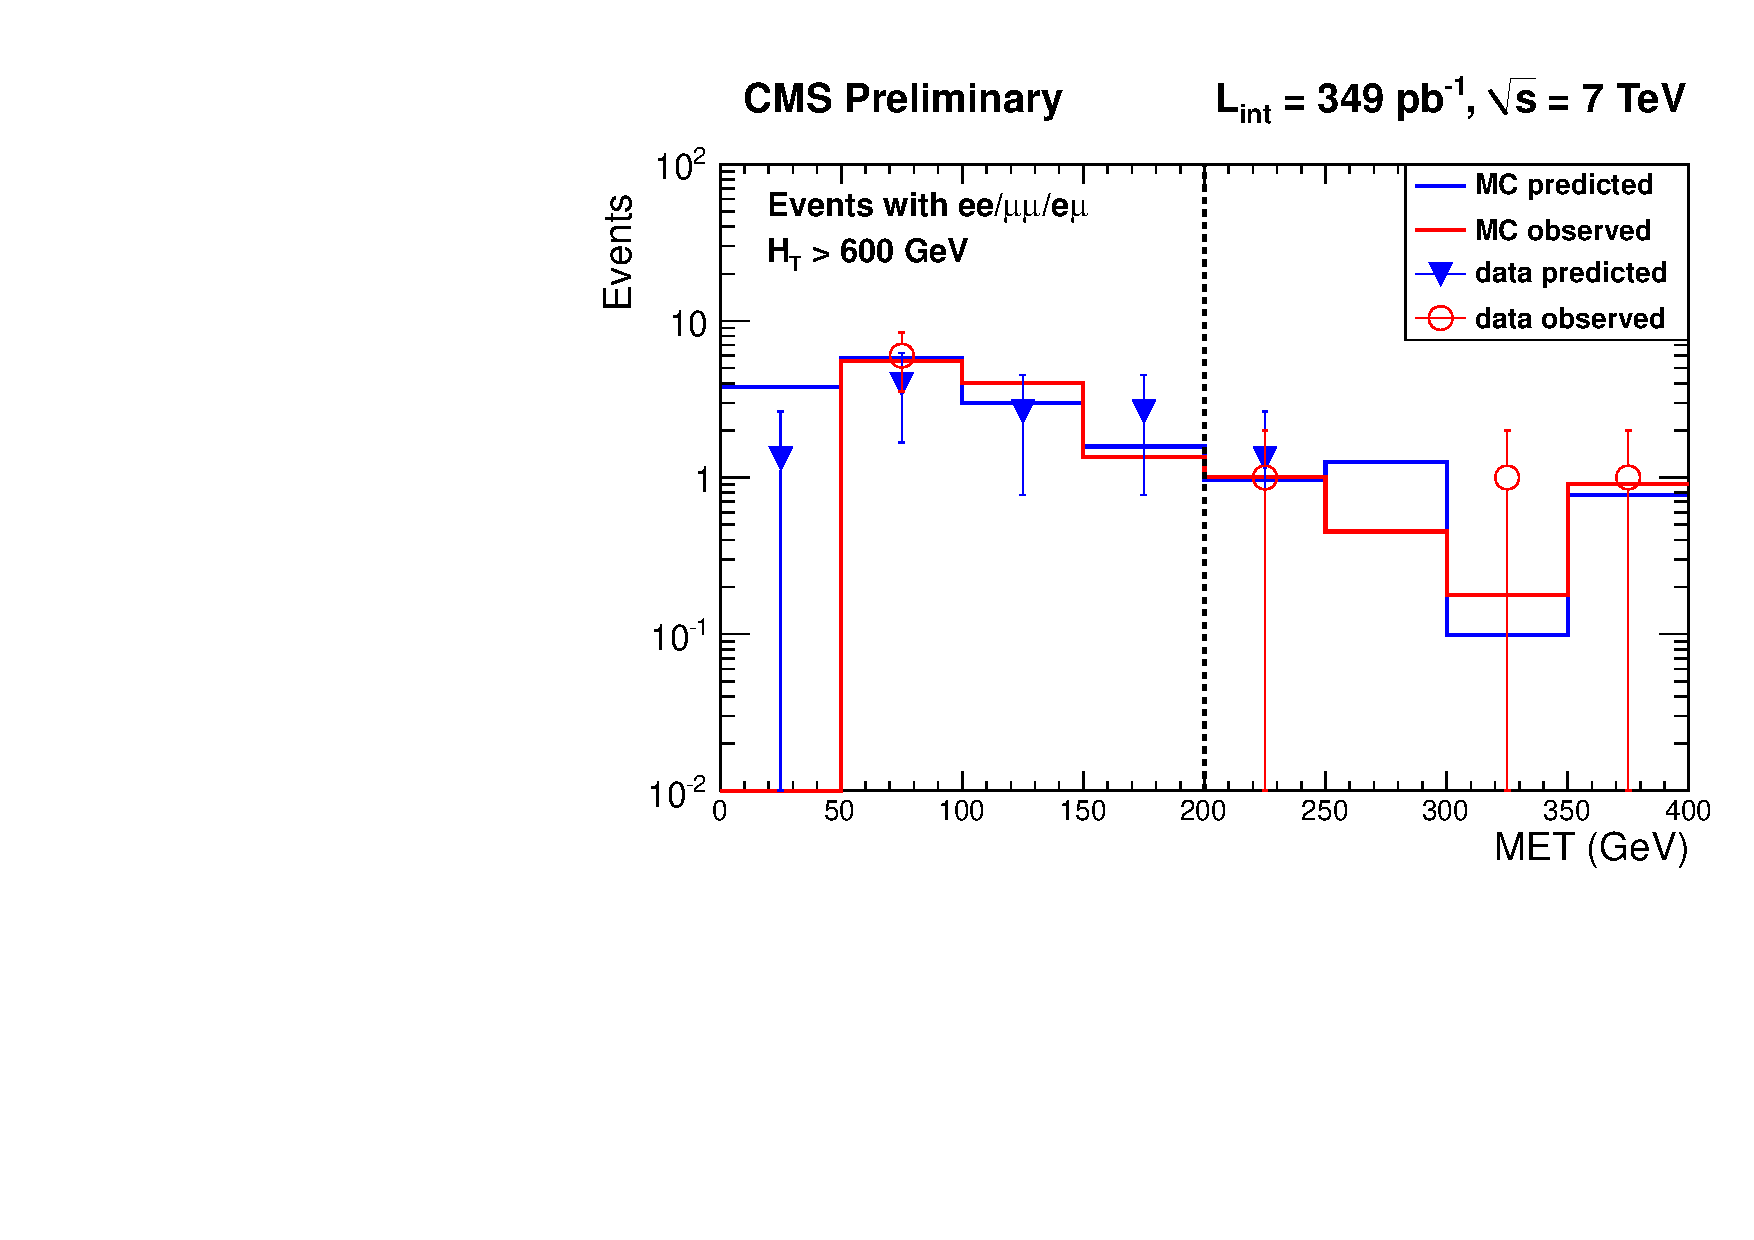
\includegraphics[width=0.48\linewidth]{plots_final/victory_met200_ht600_349pb.pdf}
\caption{\label{fig:victory}\protect 
Distributions of \ptll\ scaled by the \MET\ acceptance correction factor $K$ (predicted) 
and \met\ (observed) for SM MC and data. The high \MET\ (high \Ht) signal region
is indicated by the vertical line in the left (right) plot.
}
\end{center}
\end{figure}

The predicted and observed \MET\ distributions in the 2 signal regions are displayed
in Fig.~\ref{fig:victory}. For the high \MET\ (high \Ht) signal regions we predict
a background yield of 5.4 $\pm$ 3.8 (stat) $\pm$ 1.7 (syst) 
(1.7 $\pm$ 1.7 (stat) $\pm$ 0.4 (syst)) events, consistent with the observed yields
and with the predictions of the ABCD' method. 

As a validation of the $\pt(\ell\ell)$ method in a region which is dominated by
background, we also apply the $\pt(\ell\ell)$ method in a control region by restricting
\HT\ to be in the range 125--300~\GeV. Here we predict 6.5 $\pm$ 4.4 events with
\MET\ $>$ 200 GeV, and observe 6 events in this region.

Our third background estimate is based on the OF subtraction technique. We observe
2 $ee$ + 1 $e\mu$ (1 $ee$ + 1 $e\mu$) events in the high \MET\ (high \Ht) signal
regions outside of the $Z$ mass region 76--106~GeV. This gives 
$\Delta = $ 1.3 $\pm$ 1.9 (stat) $\pm$ 0.1 (syst) 
(0.1 $\pm$ 1.5 (stat) $\pm$ 0.0 (syst)) for the high \MET\ (high \Ht) signal regions,
respectively.

A summary of our results is presented in Table~\ref{tab:results}. For both signal regions,
the observed yield is consistent with the predictions from MC and from the background estimates
based on data. We conclude that no evidence for non-SM contributions to the signal regions
is observed.
